\section{Implementation details}
\begin{figure*}
    \centering
    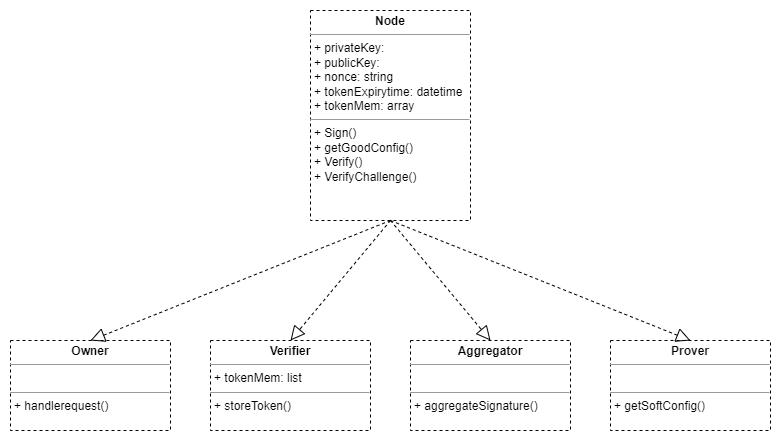
\includegraphics[width=.90\linewidth]{Images/diagramma_classi.png}  
    \caption{Class Diagram}
    \label{fig:class_diagram}
  \end{figure*}

This SANA implementation uses ''bn128'' (\cite{bn128_implementation}), an ECC implementation that uses an already existing curve belonging to the Barreto-Naherig set of curves.
This implementation uses the Barreto-Naehrig curve (\cite{barreto_naehrig}) on a finite field Zp with p of 256 bits.
The computation of the bilinear map ''bn128'' relies on the Tate-pairing technique which is the fastest for this task (\cite{tate_pairing}). It requires only one iteration of the Miller's loop function instead of three simplifying a lot the computation of the pairing.
We chose this implementation because it's a modern version of an Elliptic-curve cryptosystem used from Ethereum
It's used to generate keys, compute the signatures and verify them.
Our SANA implementation has been written and tested on python 3.7.
It defines a class for each actor in the protocol as we can see in Figure \ref{fig:class_diagram}, they all inherit from the general Node class which contains all the common data structures and functions.
On top of that the classes define:
\begin{itemize}
    \item Owner: method handlerequest() to generate the Token and generateKeys() to generate keys for the new devices.
    \item Verifier: method storeToken() to receive and store the token in the tokenMem field.
    \item Aggregator: method aggregateSignature().
    \item Prover: getSoftConfig() to retrieve its hashed software configuration.
\end{itemize}

These classes are instantiated during the simulation and each object has a set of nodes assigned as neighbors to simulate a network of devices.